\chapter{Benutzeroberfläche}

/B10/

\section{Seitenlayout}

 \begin{itemize}
   \item Bibliothek
   \begin{itemize}
    \item Suche
      \begin{itemize}
       \item Einfache Suche
       \item Erweiterte Suche
       \end{itemize}
      \item Rückgabe
      \item Einloggen
    \end{itemize}
    \item Literaturverzeichnis
    \item Administration
 \end{itemize}

\begin{itemize}
\item Fenster mit der jeweiligen Suchausgabe 
\item Anzeige, welcher Nutzer gerade aktiv ist	(falls eingeloggt)
\end{itemize}
  	 	
\begin{figure}
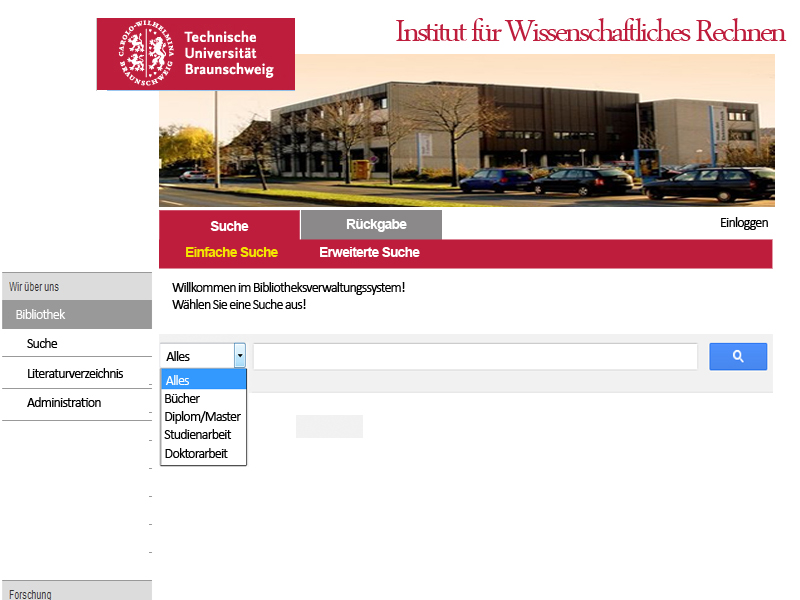
\includegraphics[width=0.8\linewidth]{bilder/layout2.jpg}
\caption[lol]{Beispiel für ein Seitenlayout}
\end{figure}


Das Beispiel (siehe Abbildung auf nächster Seite) zeigt nur den geplanten Seitenaufbau, sollte der Benutzer keinen
Account besitzen, d.h er kann lediglich die Dokumente durchsuchen.

/B20/

Darüber hinaus sind mehrere Nutzergruppen geplant:

\begin{enumerate}
\item Besucher
\item externer Benutzer
\item Normaler Benutzer
\item Bibliothekar
\item Verwaltung
\item Administrator
\end{enumerate}

Je nach Nutzergruppe verändert sich die Navigation. So erscheint bei einem Bibliothekar zusätzlich eine 
Schaltfläche „Eintragen“, mit der neu erworbene Dokumente in die Datenbank aufgenommen werden können.oder wir


/B30/

Bei einem Klick auf ein Dokument des Suchergebnisses erscheinen genauere Informationen über das Dokument (Titel,Autor,Jahr etc.), sowie
sein Status (ausgeliehen, vorhanden, verloren).

/B40/

Weiterhin ist eine Account-Verwaltungsseite geplant.
\newline
\newline
Hier kann der Nutzer, je nach Rechten:

\begin{itemize}
\item E-Mail Adresse ändern
\item sich eine Liste aller ausgeliehenen Dokumente anzeigen lassen
\item persönliche Daten ändern
\end{itemize}





 
